
\section{SPI - Serial Peripheral Interface}

\mult{2}

\begin{definition}{SPI}
SPI is a synchronous serial bus primarily for on-board connections:
\begin{itemize}
    \item Used for short-distance communication
    \item Connects microcontroller to external devices (sensors, displays, flash memory, etc.)
\end{itemize}
\end{definition}

\begin{theorem}{SPI Properties}
\begin{itemize}
    \item No defined addressing scheme (uses SS lines instead) $\rightarrow$ KISS (Keep It Simple Stupid)
    \item No built-in acknowledgment or error detection (implemented in higher-level protocols)
    \item Originally for single-byte transfers 
    \begin{itemize}
            \item $\overline{SS}$ deactivated after each byte
            \item Today also used for streams 
    \end{itemize}
    \item Flexible data rate (clock signal is transmitted with data)
    \item No flow control (master controls timing, slave cannot influence)
    \item Susceptible to noise (spikes on clock signal)
\end{itemize}
\end{theorem}

\begin{corollary}{SPI Signals}
\begin{itemize}
    \item \textbf{SCLK} (Serial Clock): Generated by master
    \item \textbf{MOSI} (Master Out Slave In)
    \item \textbf{MISO} (Master In Slave Out)
    \item \textbf{SS/CS} (Slave Select/Chip Select)
\end{itemize}
\end{corollary}

\begin{concept}{SPI Master-Slave Architecture}
\begin{itemize}
    \item Master generates common clock signal (SCLK) for all slaves
    \item Slaves: Selectable by Slave Select (SS) signal 
        \begin{itemize}
            \item Individual Select $\overline{SS1}$, $\overline{SS2}$, $\overline{SS3}$
            \item $\overline{SSx}$ = 1 $\rightarrow$ slave output MISOx is tri-state 
        \end{itemize}
    \item MOSI line connects to inputs of all slaves
    \item MISO lines from all slaves are connected to a single master input
    \item Inactive slaves (SS = '1') put their MISO line in tri-state (high impedance)
    \item Only one selected slave drives its MISO line at a time
\end{itemize}
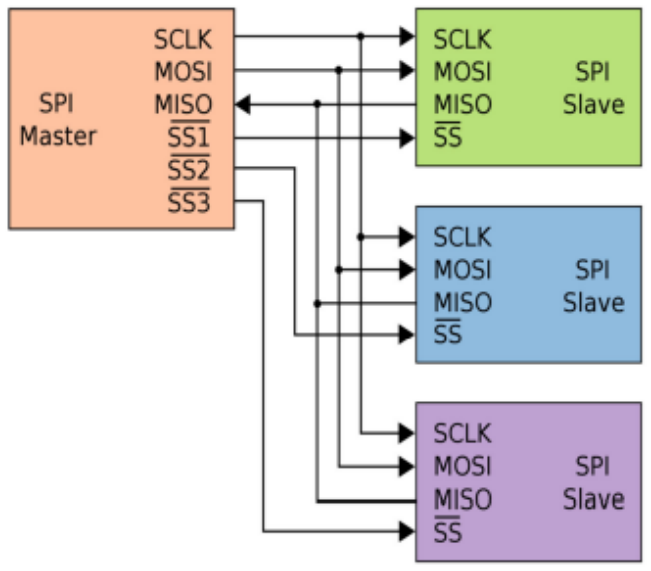
\includegraphics[width=0.7\linewidth]{single_master_mult_slaves.png}
\end{concept}

\multend

\begin{definition}{SPI Implementation Using Shift Registers}
\begin{itemize}
    \item Both master and slave contain 8-bit shift registers
    \item Bits are shifted out on one clock edge (toggling edge)
    \item Bits are sampled on the other clock edge (sampling edge)
    \item 8 clock cycles exchange 8 bits in each direction simultaneously
    \item After 8 clock cycles, data has been exchanged in both directions
    \item Status flags (TXE, RXNE) indicate buffer status
\end{itemize}
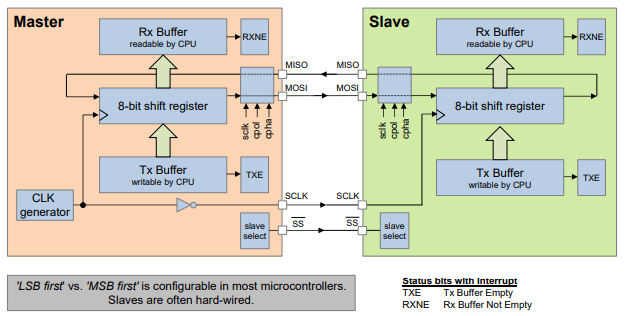
\includegraphics[width=\linewidth]{spi_impleemtation.png}
\end{definition}




\subsection{SPI Modes and Timing}

\begin{definition}{SPI Timing}\\
    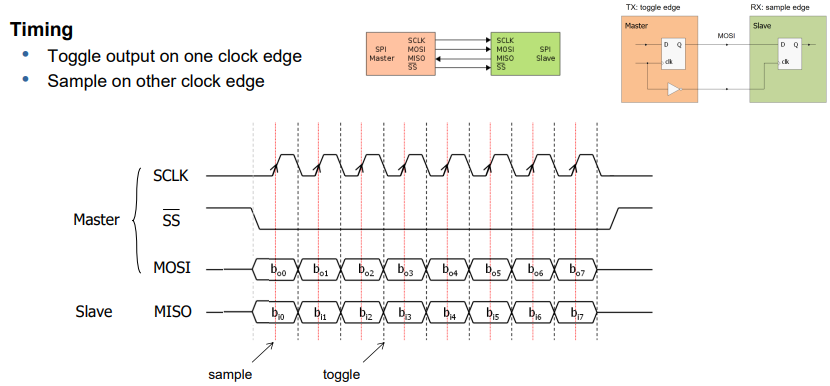
\includegraphics[width=\linewidth]{spi_timing_overview.png}
\end{definition}

\begin{concept}{Clock Polarity and Phase}
SPI has four different modes based on two parameters:

\begin{minipage}{0.5\linewidth}
\textbf{CPOL} (Clock Polarity): Idle state of clock
    \begin{itemize}
        \item CPOL = 0: Clock idles at low level
        \item CPOL = 1: Clock idles at high level
    \end{itemize}
\end{minipage}
\begin{minipage}{0.5\linewidth}
\textbf{CPHA} (Clock Phase): Which edge is used for data sampling
    \begin{itemize}
        \item CPHA = 0: Data sampled on first clock edge
        \item CPHA = 1: Data sampled on second clock edge
    \end{itemize}
\end{minipage}
\end{concept}

\begin{concept}{Four SPI Modes}

\begin{minipage}{0.5\linewidth}
\textbf{Mode 0}: CPOL = 0, CPHA = 0
    \begin{itemize}
        \item Clock idles low
        \item Data sampled on rising edge, changed on falling edge
    \end{itemize}
\textbf{Mode 1}: CPOL = 0, CPHA = 1
    \begin{itemize}
        \item Clock idles low
        \item Data sampled on falling edge, changed on rising edge
    \end{itemize}
\end{minipage}
\begin{minipage}{0.5\linewidth}
\textbf{Mode 2}: CPOL = 1, CPHA = 0
    \begin{itemize}
        \item Clock idles high
        \item Data sampled on falling edge, changed on rising edge
    \end{itemize}
\textbf{Mode 3}: CPOL = 1, CPHA = 1
    \begin{itemize}
        \item Clock idles high
        \item Data sampled on rising edge, changed on falling edge
    \end{itemize}
\end{minipage}
\end{concept}

\begin{center}
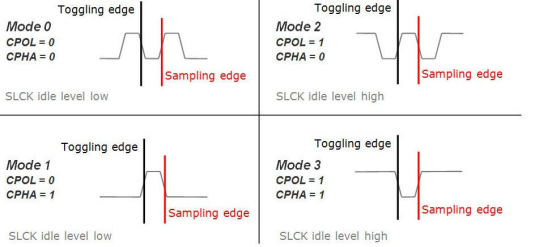
\includegraphics[width=0.75\linewidth]{spi_timing_kr.png}
\end{center}


\begin{KR}{SPI Timing-Diagramm zeichnen}

    \begin{minipage}{0.6\linewidth}
    \paragraph{SPI-Modi (CPOL/CPHA)}
    \begin{itemize}
        \item Mode 0: CPOL=0, CPHA=0 (Idle=Low, Sample=Rising)
        \item Mode 1: CPOL=0, CPHA=1 (Idle=Low, Sample=Falling)
        \item Mode 2: CPOL=1, CPHA=0 (Idle=High, Sample=Falling)
        \item Mode 3: CPOL=1, CPHA=1 (Idle=High, Sample=Rising)
    \end{itemize}
    \end{minipage}
    \hspace{2mm}
    \begin{minipage}{0.35\linewidth}    
    \paragraph{Signale}
    \begin{itemize}
        \item SS (Slave Select): \\ aktiv-low, Slave-Auswahl
        \item SCLK: Clock vom Master
        \item MOSI: Master Out Slave In
        \item MISO: Master In Slave Out
    \end{itemize}
    \end{minipage}
    
    \paragraph{Timing zeichnen}

    \begin{minipage}{0.6\linewidth}
    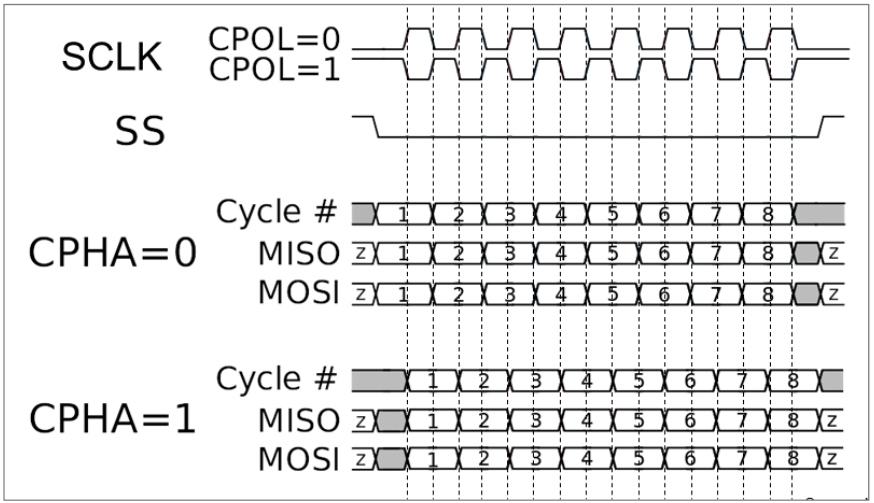
\includegraphics[width=\linewidth]{SPI_communication.png}
    \end{minipage}
    \begin{minipage}{0.35\linewidth}
    \begin{enumerate}
        \item SCLK entsprechend CPOL \\ (Idle-Level)
        \item SS aktiv (low) \\ für gesamte Übertragung
        \item Daten auf MOSI/MISO je nach CPHA (Toggling Edge)
        \item MOSI: Data from Master to Slave
        \item MISO: Data from Slave to Master
        \item Sampling Edges markieren basierend auf CPHA
    \end{enumerate}
    \end{minipage}

    \paragraph{Calculate timing parameters}
    \begin{itemize}
        \item Bit cell time = 1/clock\_frequency
        \item Frame time = (number\_of\_bits)/clock\_frequency
        \item Example: 8 bits at 100 kHz = 80 µs per frame
    \end{itemize}

\end{KR}

\begin{example2}{SPI Mode 3 Timing}\\
    \begin{minipage}{0.5\linewidth}
    SPI Interface mit 8 Bit Daten:
    \begin{itemize}
        \item MOSI: 0xA7 (10100111b)
        \item MISO: 0x37 (00110111b)
    \end{itemize}
    \end{minipage}
    \begin{minipage}{0.5\linewidth}
    \begin{itemize}
        \item Mode 3: CPOL=1, CPHA=1
        \item MSB first
        \item SCLK: 100kHz
    \end{itemize}
    \end{minipage}
    
    \textbf{Timing-Diagramm:}
    \begin{center}
    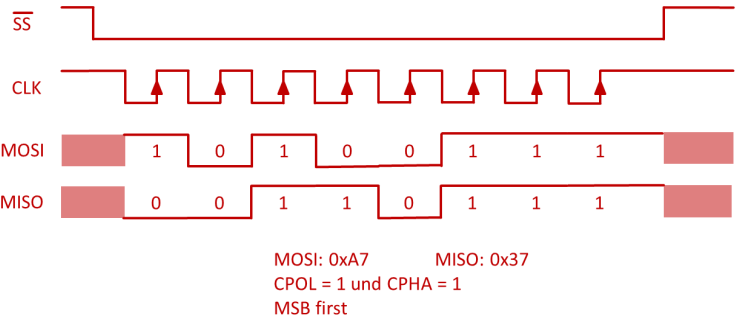
\includegraphics[width=0.8\linewidth]{spi_timing_ex.png}
    \end{center}

    \begin{minipage}{0.5\linewidth}
        \textbf{Timing-Charakteristika:}
    \begin{itemize}
        \item SCLK Idle = High (CPOL=1)
        \item Daten wechseln auf steigende Flanke (CPHA=1)
        \item Sampling auf fallende Flanke
        \item Bit-Zeit = 1/100kHz = 0.01 ms = 10 $\mu$s
    \end{itemize}
    \end{minipage}
    \begin{minipage}{0.5\linewidth}
        \textbf{Daten-Übertragung:}
    \begin{itemize}
        \item SS: Low waehrend gesamter Uebertragung
        \item SCLK: startet High, 8 Taktzyklen
        \item MOSI: 1-0-1-0-0-1-1-1 (MSB first)
        \item MISO: 0-0-1-1-0-1-1-1 (MSB first)
    \end{itemize}
    \end{minipage}
\end{example2}

\begin{remark}
    Bei SPI ist die Uebertragung immer full-duplex - Master und Slave senden gleichzeitig. Auch wenn nur in eine Richtung Daten benoetigt werden, findet auf der anderen Leitung eine "Dummy"-Uebertragung statt.
\end{remark}









\subsection{SPI Implementation}





\begin{concept}{STM32 SPI Architecture}\\
The STM32F4 SPI peripheral includes:
\begin{itemize}
    \item Configuration registers (SPI\_CR1, SPI\_CR2)
    \item Status register (SPI\_SR)
    \item Data register (SPI\_DR) for transmit and receive
    \item Status flags for synchronization (TXE, RXNE, BSY)
    \item Support for different communication modes
    \item DMA capability for high-speed transfers
\end{itemize}
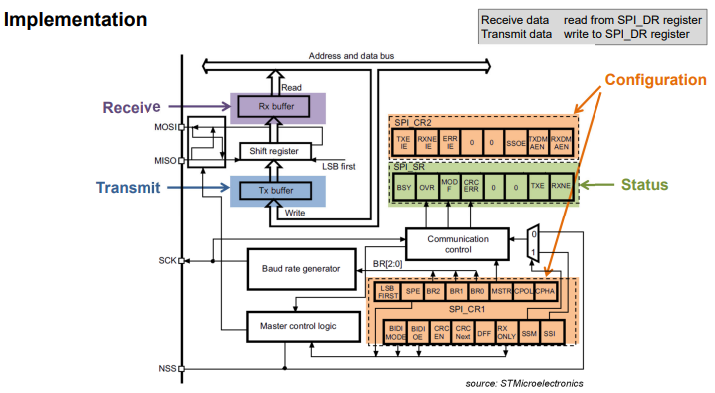
\includegraphics[width=\linewidth]{spi_implementation.png}
\end{concept}


\begin{theorem}{Synchronizing Hardware and Software} 
    When shall software access the shift register?\\
    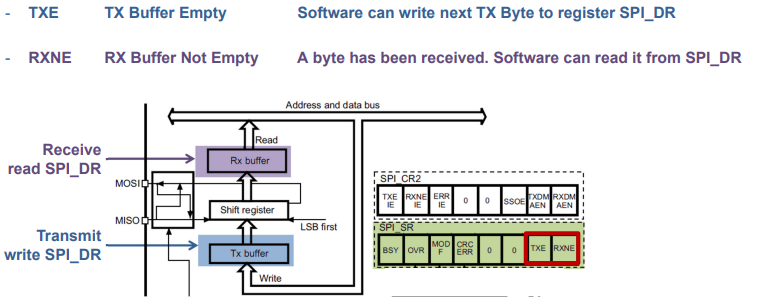
\includegraphics[width=\linewidth]{spi_synchonozing.png}
\end{theorem}

\begin{KR}{Simultaneously Handling Data Transmission and Reception}
    Full Duplex: Check TXE (Transmit Buffer Empty) and RXNE (Receive Buffer Not Empty) flags to manage data flow.\\
    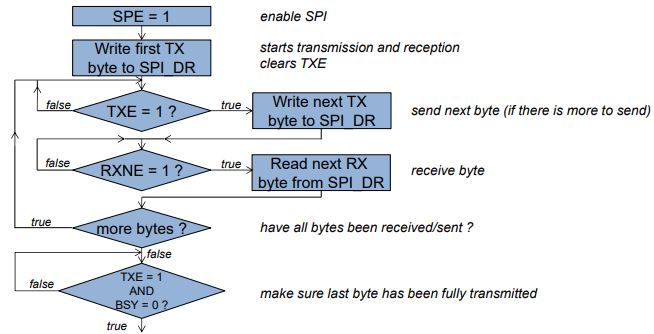
\includegraphics[width=0.8\linewidth]{spi_simult_handling.png}
\end{KR}

\begin{corollary}{Synchronizing Hardware and Software}
    \begin{itemize}
        \item TXE (TX Buffer Empty) $\rightarrow$ Software can write next TX Byte to SPI\_DR
        \item RXNE (RX Buffer Not Empty) $\rightarrow$ a byte has been received. Software can read it from SPI\_DR
        \item BSY (Busy) $\rightarrow$ Transmission in progress
    \end{itemize}
    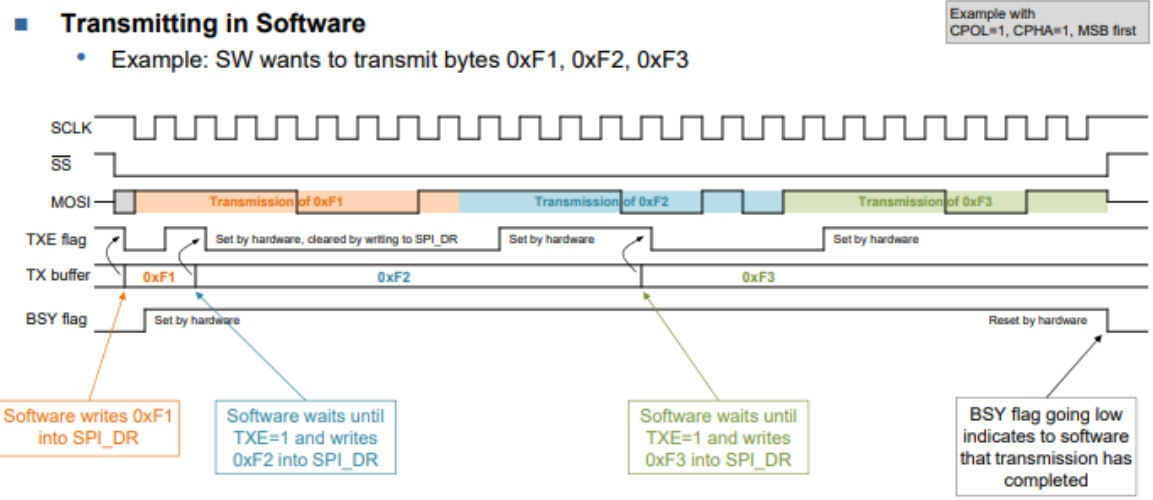
\includegraphics[width=\linewidth]{transmitting_spi.png}\\
    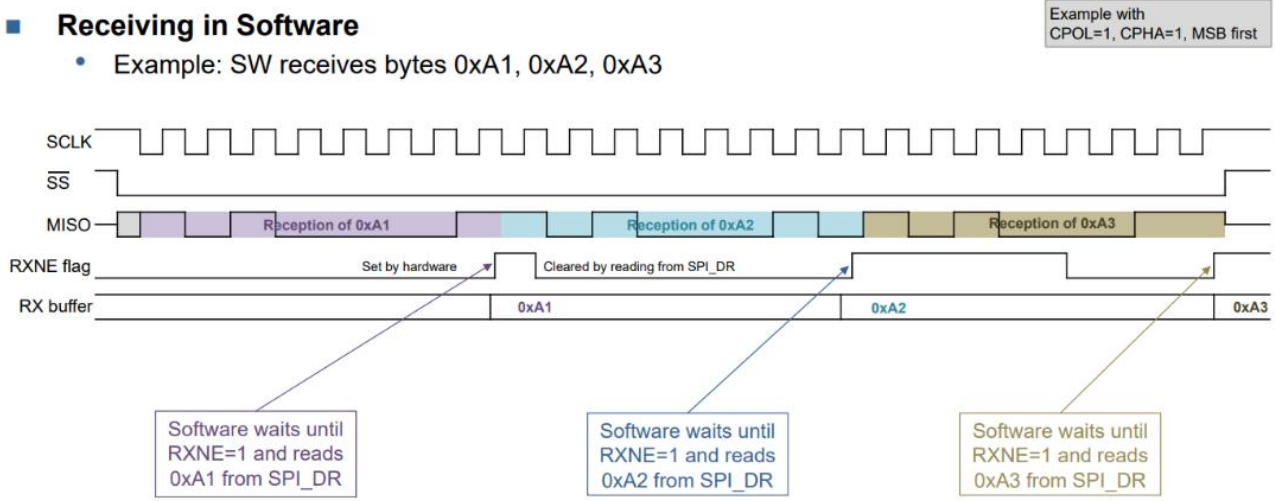
\includegraphics[width=\linewidth]{receiving_spi.png}
\end{corollary}



\subsubsection{STM32 SPI Configuration and Usage}

\begin{definition}{STM32 SPI Registers}\\
    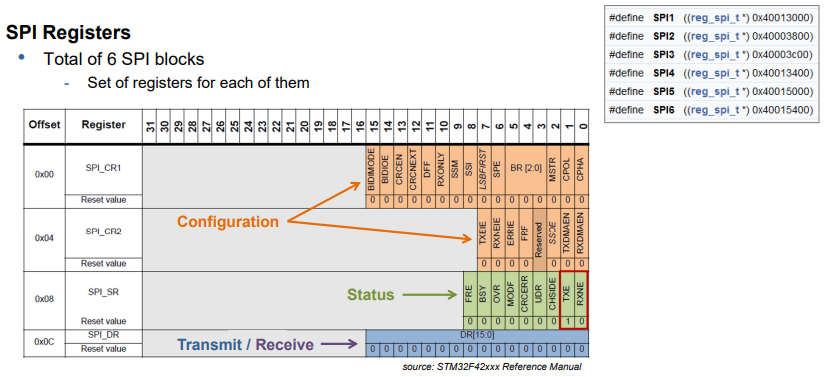
\includegraphics[width=\linewidth]{spi_registers.png}
\end{definition}

\begin{concept}{SPI Register Bits}\\
    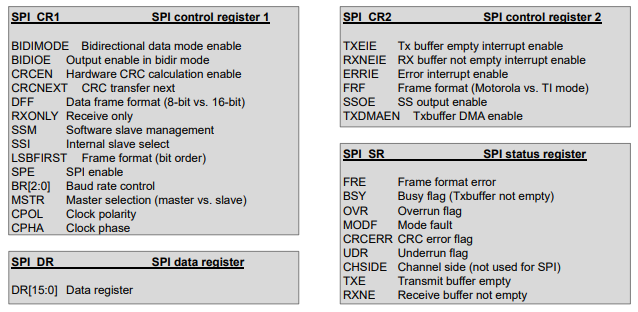
\includegraphics[width=\linewidth]{spi_register_bits.png}
\end{concept}

\begin{code}{STM32 SPI Register Configuration}
\begin{lstlisting}[language=C, style=basesmol]
// SPI configuration example
// Configure SPI1 in master mode, CPOL=1, CPHA=1, 8-bit data

// Enable SPI1 clock
RCC->APB2ENR |= RCC_APB2ENR_SPI1EN;

// Configure SPI1
SPI1->CR1 = (1 << 0)   // CPHA=1
          | (1 << 1)   // CPOL=1
          | (1 << 2)   // Master mode
          | (3 << 3)   // BR[2:0]=011: fPCLK/16 (prescaler)
          | (0 << 7)   // MSB first (LSBFIRST=0)
          | (1 << 8)   // SSI=1 (needed for software SS)
          | (1 << 9);  // SSM=1 (software slave management)

// Enable SPI
SPI1->CR1 |= (1 << 6); // SPE=1 (SPI enable)
\end{lstlisting}
\end{code}

\begin{KR}{Transmitting Data with SPI}
\paragraph{Step 1: Prepare SPI}
Configure and enable the SPI peripheral.
\paragraph{Step 2: Check TXE flag}
Wait until the transmit buffer is empty.
\paragraph{Step 3: Write data}
Write data to the data register.
\paragraph{Step 4: Wait for completion}
Wait until transmission is complete by checking BSY flag.

\begin{lstlisting}[language=C, style=basesmol]
// Transmit a byte over SPI
uint8_t transmit_byte(uint8_t data) {
    // Step 1: SPI should already be configured
    
    // Step 2: Wait until TXE=1 (transmit buffer empty)
    while (!(SPI1->SR & (1 << 1))) { }
    
    // Step 3: Write data to transmit
    SPI1->DR = data;
    
    // Step 4: Wait for reception (needed to get received data)
    while (!(SPI1->SR & (1 << 0))) { }
    
    // Return received data (read DR clears RXNE flag)
    return SPI1->DR;
}
\end{lstlisting}
\end{KR}

\begin{KR}{Handling Full-Duplex SPI Communication}
    \begin{enumerate}
        \item Enable SPI with SPE bit: Ensure SPI is properly configured and enabled.
        \item Write first byte to transmit: Write the first byte to the data register (DR) to start transmission/reception.
        \item Process data in a loop: Check TXE (Transmit Buffer Empty) and RXNE (Receive Buffer Not Empty) flags to handle both transmission and reception.
        \item Wait for completion: Wait for BSY (Busy) flag to be cleared, indicating that all transfers are complete.
    \end{enumerate}

\begin{lstlisting}[language=C, style=basesmol]
void spi_transfer(uint8_t *tx_data, uint8_t *rx_data, uint16_t length) {
    // Enable SPI
    SPI1->CR1 |= (1 << 6);  // SPE=1
    if (length > 0) { // Write first TX byte to start transmission
        SPI1->DR = tx_data[0];
    }
    uint16_t tx_count = 1;
    uint16_t rx_count = 0;
    while (rx_count < length) { // Process data
        // Check if we can transmit more data
        if ((tx_count < length) && (SPI1->SR & (1 << 1))) {  // TXE=1
            SPI1->DR = tx_data[tx_count++];
        }
        // Check if we received data
        if (SPI1->SR & (1 << 0)) {  // RXNE=1
            rx_data[rx_count++] = SPI1->DR;
        }
    }
    while (SPI1->SR & (1 << 7)) { } // Wait until BSY=0 (SPI not busy)
}
\end{lstlisting}
\end{KR}

\subsubsection{SPI Flash Devices} 

\begin{definition}{Save Board Area}
    Example: Micron M25PE40 Serial Flash Memory
    \begin{itemize}
        \item 4 Mbit NOR Flash
        \item 6 x 5 mm package size
        \item SCLK: up to 75 MHz
    \end{itemize}

    \begin{minipage}{0.5\linewidth}
        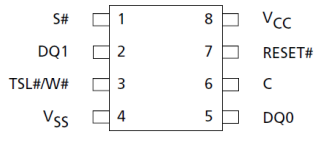
\includegraphics[width=\linewidth]{spi_flash1.png}
    \end{minipage}
    \begin{minipage}{0.5\linewidth}
        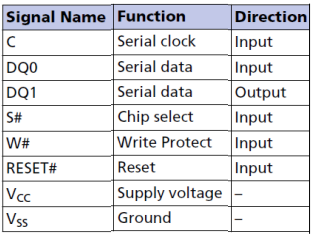
\includegraphics[width=\linewidth]{spi_flash2.png}
    \end{minipage}
\end{definition}


    